\documentclass[11pt,aspectratio=169]{beamer}
% \usepackage[UTF8]{ctex}

\usetheme[progressbar=frametitle]{metropolis}
\usepackage{appendixnumberbeamer}
\usepackage{amsmath,bm}

\usepackage{booktabs}
\usepackage[scale=2]{ccicons}
\usepackage{hyperref}
\usepackage{gensymb}
\usepackage{xspace}
\usepackage{pgfplots}
\usepackage{textpos}
\usepackage{svg}
\usepackage{listings}
\usepackage{ragged2e}

\usepackage{xcolor}

\definecolor{codegreen}{rgb}{0,0.6,0}
\definecolor{codegray}{rgb}{0.5,0.5,0.5}
\definecolor{codepurple}{rgb}{0.58,0,0.82}
\definecolor{backcolour}{rgb}{0.95,0.95,0.92}

\lstdefinestyle{mystyle}{
    backgroundcolor=\color{backcolour},   
    commentstyle=\color{codegreen},
    keywordstyle=\color{magenta},
    numberstyle=\tiny\color{codegray},
    stringstyle=\color{codepurple},
    basicstyle=\ttfamily\footnotesize,
    breakatwhitespace=false,         
    breaklines=true,                 
    captionpos=b,                    
    keepspaces=true,                 
    numbers=left,                    
    numbersep=5pt,                  
    showspaces=false,                
    showstringspaces=false,
    showtabs=false,                  
    tabsize=2
}

\lstset{style=mystyle}


% \usepackage{helvet}

% \usepackage{enumitem}
% \usepackage[para]{footmisc}

\usepgfplotslibrary{dateplot}

\newcommand{\STO}{$\mathsf{SrTiO_3}$\xspace}
\newcommand{\BFO}{$\mathsf{BiFeO_3}$\xspace}
\newcommand{\BTO}{$\mathrm{BiTiO_3}$\xspace}
\newcommand{\PTO}{$\mathrm{PbTiO_3}$\xspace}
\newcommand{\degreex}{\degree\xspace}



\definecolor{psu-palette-slate}{HTML}{314D64}
\definecolor{psu-palette-creek}{HTML}{3EA39E}
\definecolor{psu-palette-limestone}{HTML}{91959C}
\definecolor{psu-palette-sky}{HTML}{009CDE}
\definecolor{psu-palette-blue}{HTML}{1E407C}
\definecolor{psu-palette-navy}{HTML}{001E44}

\definecolor{psu-vibrant-dawn}{HTML}{f2665e}
\definecolor{psu-vibrant-orange}{HTML}{E98300}
\definecolor{psu-vibrant-keystone}{HTML}{FFD100}
\definecolor{psu-vibrant-green}{HTML}{008755}
\definecolor{psu-vibrant-perpetual}{HTML}{491d70}
\definecolor{psu-vibrant-future}{HTML}{99cc00}

\setbeamercolor{palette primary}{bg=psu-palette-navy}
\setbeamercolor{title separator}{fg=psu-palette-navy}
\setbeamercolor{progress bar}{fg=psu-palette-sky,bg=psu-palette-blue}
\setbeamercolor{progress bar in head/foot}{fg=psu-vibrant-dawn,bg=psu-vibrant-orange}
\setbeamercolor{alerted text}{fg=red}

\usepackage{xspace}
\newcommand{\themename}{\textbf{\textsc{metropolis}}\xspace}

\title{Introduction to the Phase-Field Method and Its Applications}
\subtitle{Hands on tutorials and exercises}
% \date{\today}
\date{ June, 24th, 2020}
\author{Xiaoxing Cheng}
\institute{Materials Science and Engineering, The Pennsylvania State University}
% \titlegraphic{\hfill
\includegraphics[height=1.5cm]{logo.pdf}}

\usebackgroundtemplate{
% 
\includegraphics[width=\paperwidth]{bg.png}
\tikz\node[opacity=0.10] {
\includegraphics[width=\paperwidth]{lion_bg}};
}

\addtobeamertemplate{frametitle}{}{%
% \vskip -0.95cm
% \includegraphics[height=0.8cm]{lgog.png}
% \vskip 0.95cm
\begin{textblock*}{100mm}(.85\textwidth,-0.95cm)

\includegraphics[height=0.8cm]{logo.png}
\end{textblock*}
% \begin{tikzpicture}[remember picture,overlay]
% \node[anchor=north east,yshift=0.2ex] at (current page.north east) {
\includegraphics[height=0.8cm]{logo.png}};
% \end{tikzpicture}
}

% \makeatletter
% \define@key{beamerframe}{t}[true]{% top
%   \beamer@frametopskip=.2cm plus .5\paperheight\relax%
%   \beamer@framebottomskip=0pt plus 1fill\relax%
%   \beamer@frametopskipautobreak=\beamer@frametopskip\relax%
%   \beamer@framebottomskipautobreak=\beamer@framebottomskip\relax%
%   \def\beamer@initfirstlineunskip{}%
% }
% \makeatother  

\makeatletter
\renewcommand\@makefntext[1]{%
   \noindent
%   \makebox[0pt][r]{\@thefnmark.\space}
   #1
   }
\makeatother

\begin{document}

\newcommand\fnl{}
\newcommand\nothing{}
% \renewcommand\fnl{doi:10.1007/s10832-007-9120-8, doi:10.1088/0268-1242/20/4/006, doi:10.1126/science.1129564, doi:10.1063/1.5116910}

\setbeamertemplate{footline}[text line]{%
  \parbox{0.85\linewidth}{
    \vspace*{-8pt}  
    \ifx \fnl \nothing
        \message{\fnl is defined}
    \else
    \footnoterule 
    \fi \fnl%
  }
  \hfill%
  \parbox{0.15\linewidth}{
    \vspace*{-8pt}\raggedleft\insertframenumber %\insertpagenumber
  }
}
    
    
    
\maketitle

\begin{frame}{Outline}
  \setbeamertemplate{section in toc}[sections numbered]
  \vskip 0.5cm
  \tableofcontents%[hideallsubsections]
\end{frame}

\section[MUPRO]{MUPRO}
\begin{frame}{MUPRO}
\begin{columns}
\column{.45\linewidth}

\includegraphics[width=\textwidth]{img/text.png}
\column{.55\linewidth}
\begin{center}
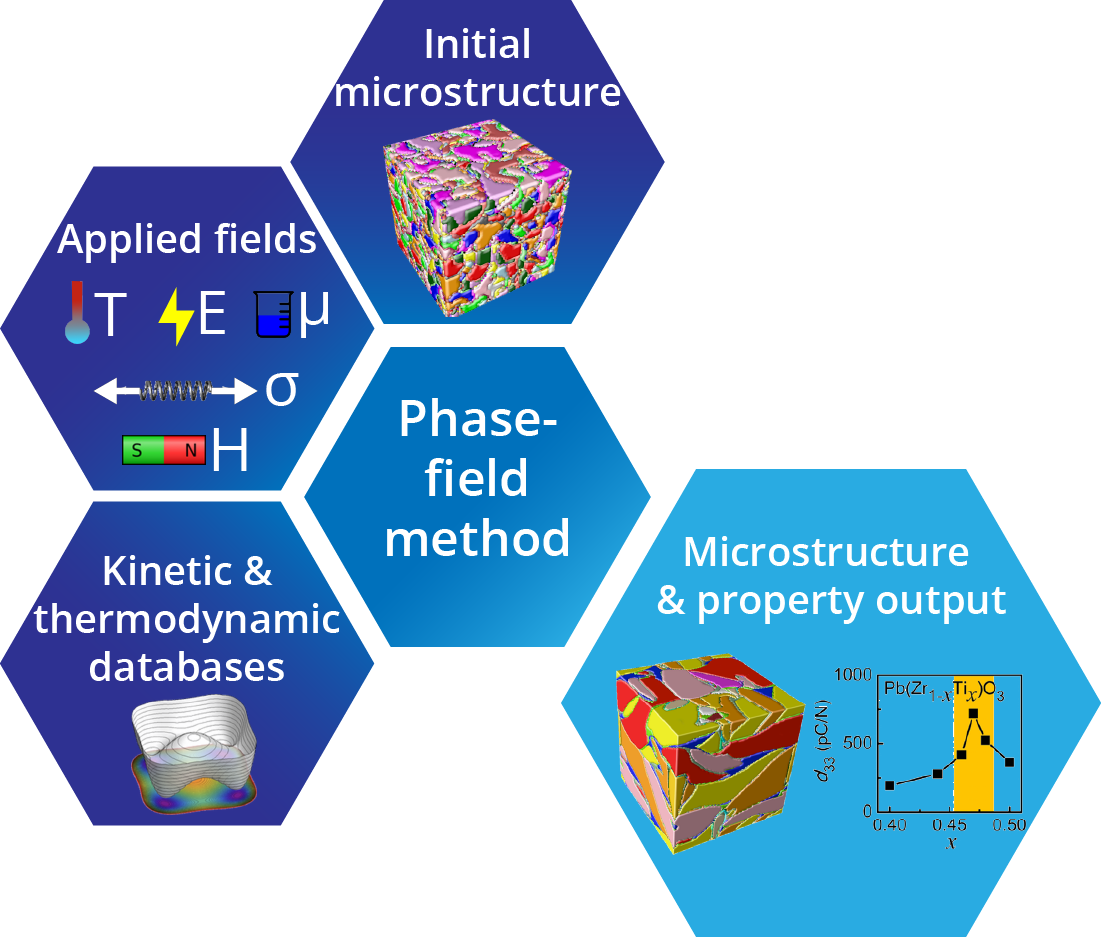
\includegraphics[width=\textwidth]{img/phase-field.png}
\end{center}
\end{columns}
\end{frame}

\section[Part One: Tutorials]{Part One: Tutorials}
% \subsection[Ferroelectrics]{Ferroelectrics}

\begin{frame}[fragile]{Preparation}
\begin{columns}[t]
\column{0.6\linewidth}
Connect to the online portal: \href{portal.aci.ics.psu.edu}{portal.aci.ics.psu.edu}
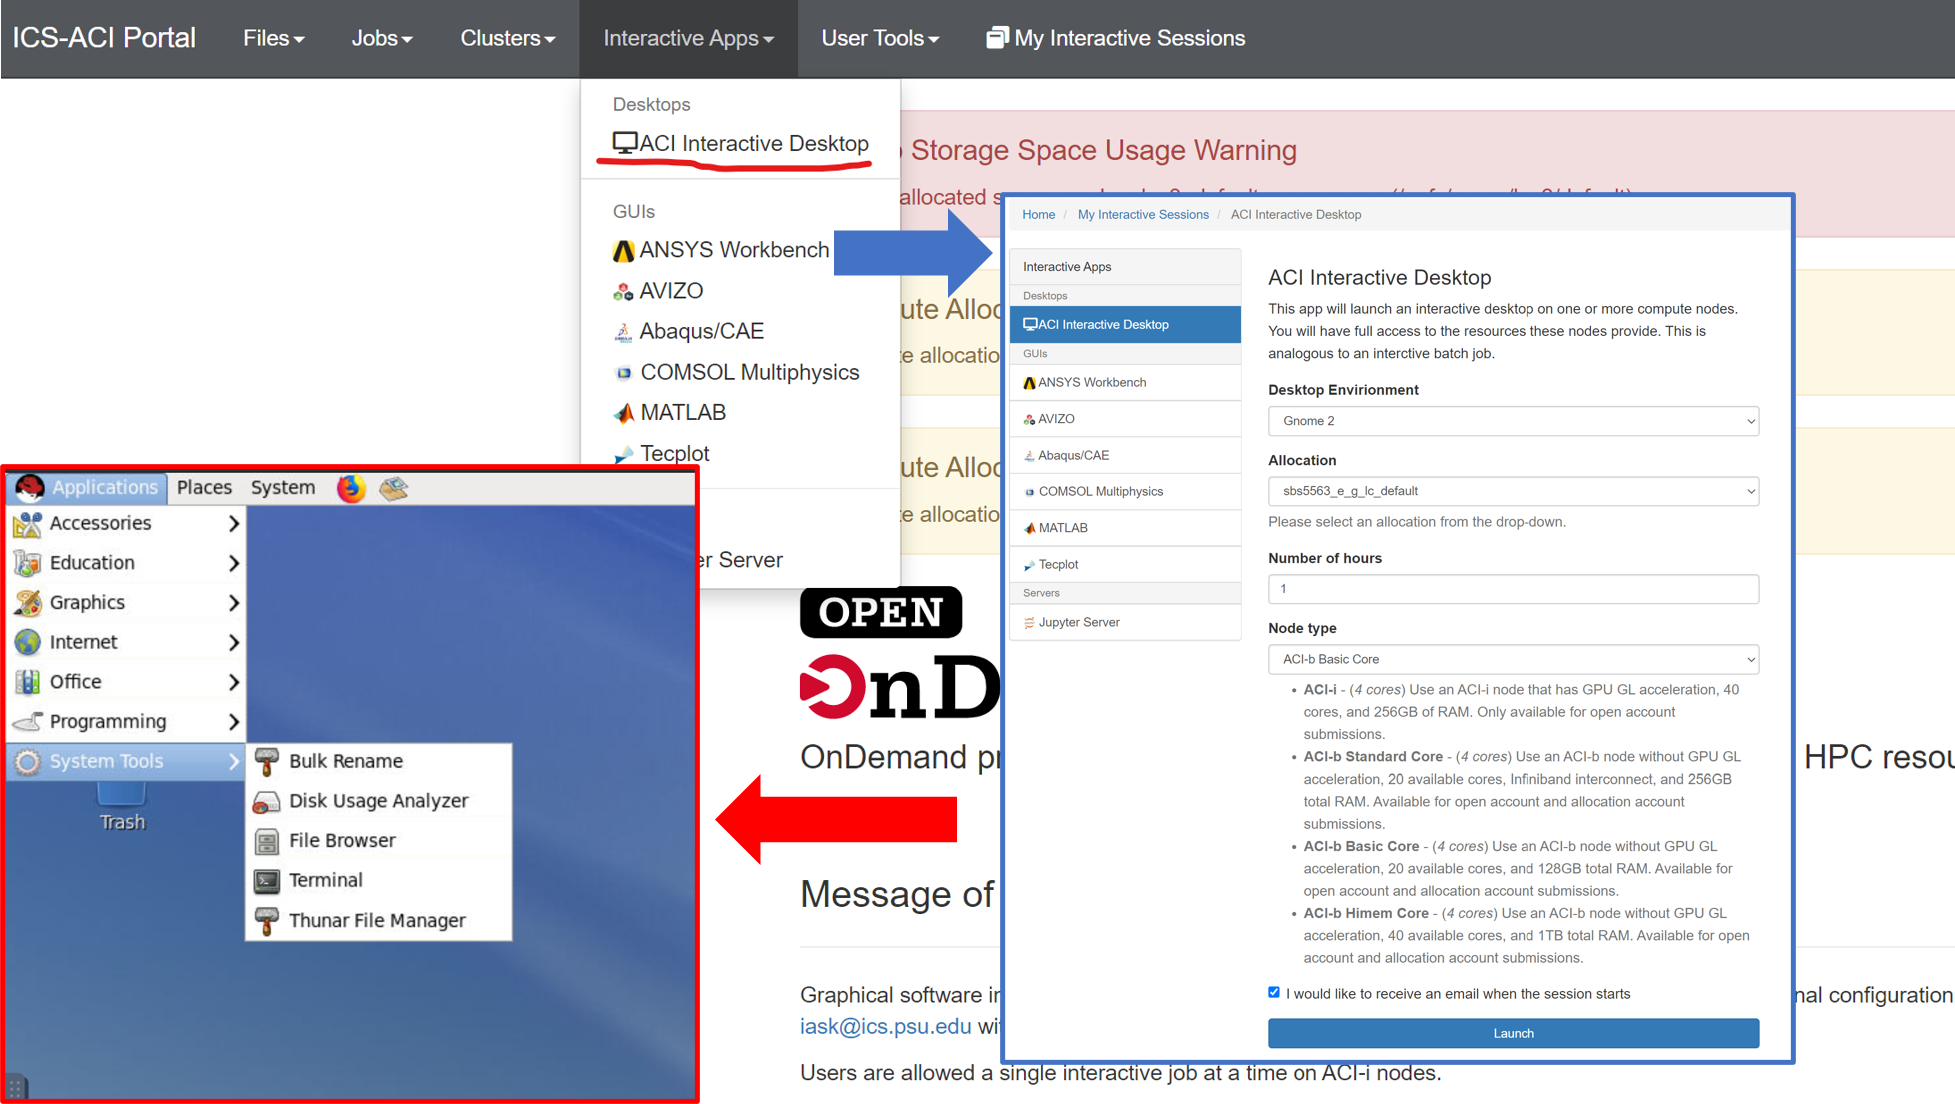
\includegraphics[width=0.9\linewidth]{img/interactive-allocation.png}
\column{0.3\linewidth}
Most used commands\\
\begin{itemize}
    \item [{\bf ls}] list directory
    \item [{\bf cd}] change directory
    \item [{\bf cp}] copy
    \item [{\bf mkdir}] make directory
    \item [{\bf module list}] loaded modules
    \item [{\bf module avail}] available modules
    \item [{\bf module load}] load module
    \item [{\bf qsub }] submit job 
    \item [{\bf qstat }] status of job
\end{itemize}
\end{columns}

\end{frame}
\begin{frame}[fragile]{Preparation}
\begin{columns}
\column{0.9\linewidth}
\begin{lstlisting}[language=bash]
cd ~/scratch # Go to your scratch folder
mkdir pfm    # Create a folder for the tutorial
cd pfm       # Go into the created folder
module load python/3.6.3-anaconda5.0.1
cp -r /gpfs/group/dml129/default/matse_sc_data/lchen/doc .
\end{lstlisting}
\end{columns}
\end{frame}

\subsection[Project 1: Ferroelectric]{Project 1: Ferroelectric}
\begin{frame}[fragile]{Project 1: Ferroelectric -- Preparation}
\small{
\begin{lstlisting}[language=bash]
cp -r /gpfs/group/dml129/default/matse_sc_data/lchen/project1 .
cd project1
ls
\end{lstlisting}
}
\begin{columns}
\column{0.7\linewidth}
    \begin{itemize}
        \item [input.in] Boundary conditions and applied external field 
        \item [pot.in] Thermodynamic and physical properties of the material
        \item [ferro.pbs] The PBS submission script
        \item [Ferroelectric.exe] The executable that we are using
    \end{itemize}
    % \vskip 0.5cm
    % Polar.in may also be defined for customizing the initial polarization distribution.
\end{columns}
\end{frame}

\renewcommand\fnl{doi: 10.1146/annurev-matsci-071312-121634, doi: 10.1063/1.5116910, doi: 10.1002/adfm.201801725 }
% \subsection[Phase-field model]{Phase-field model}
\begin{frame}[t]{Phase-field model}
\begin{columns}[T]
\column{0.7\linewidth}
\begin{flalign*}
\only<1>{& \frac{\partial \eta}{\partial t} = -L \frac{\delta F}{\delta \eta} \\}
\only<2->{& \frac{\partial \eta}{\partial t} = -L \frac{\delta F}{\delta \eta}, \quad F =}
\only<2>{\int_\Omega ({\color{red}f_{land}+f_{grad}})d\Omega \\}
\only<3>{\int_\Omega (f_{land}+f_{grad}+{\color{red}f_{elas}})d\Omega \\}
\only<4>{\int_\Omega (f_{land}+f_{grad}+f_{elas}+{\color{red}f_{elec}})d\Omega \\}
\only<2->{& \alert<2>{f_{land}(\bm{p}) = \alpha_{i}p_i^2+\alpha_{ij}p_i^2p_j^2+\alpha_{ijk}p_i^2p_j^2p_k^2} \\
& \alert<2>{f_{grad}(\bm{p}) = \frac{1}{2} G^p_{ijkl}p_{i,j}p_{k,l}}\\}
\only<3->{   & \alert<3>{f_{elas}(\bm{p},\bm{\epsilon}) = \frac{1}{2}C_{ijkl}(\epsilon_{ij}-\epsilon_{ij}^0)(\epsilon_{kl}-\epsilon_{kl}^0)} \\}
\only<4->{   & \alert<4>{f_{elec}(\bm{p},\bm{E}) = -\frac{1}{2}\epsilon_0E_iE_j-E_ip_i}}
\end{flalign*}
\column{0.3\linewidth}
\only<2>{\centering 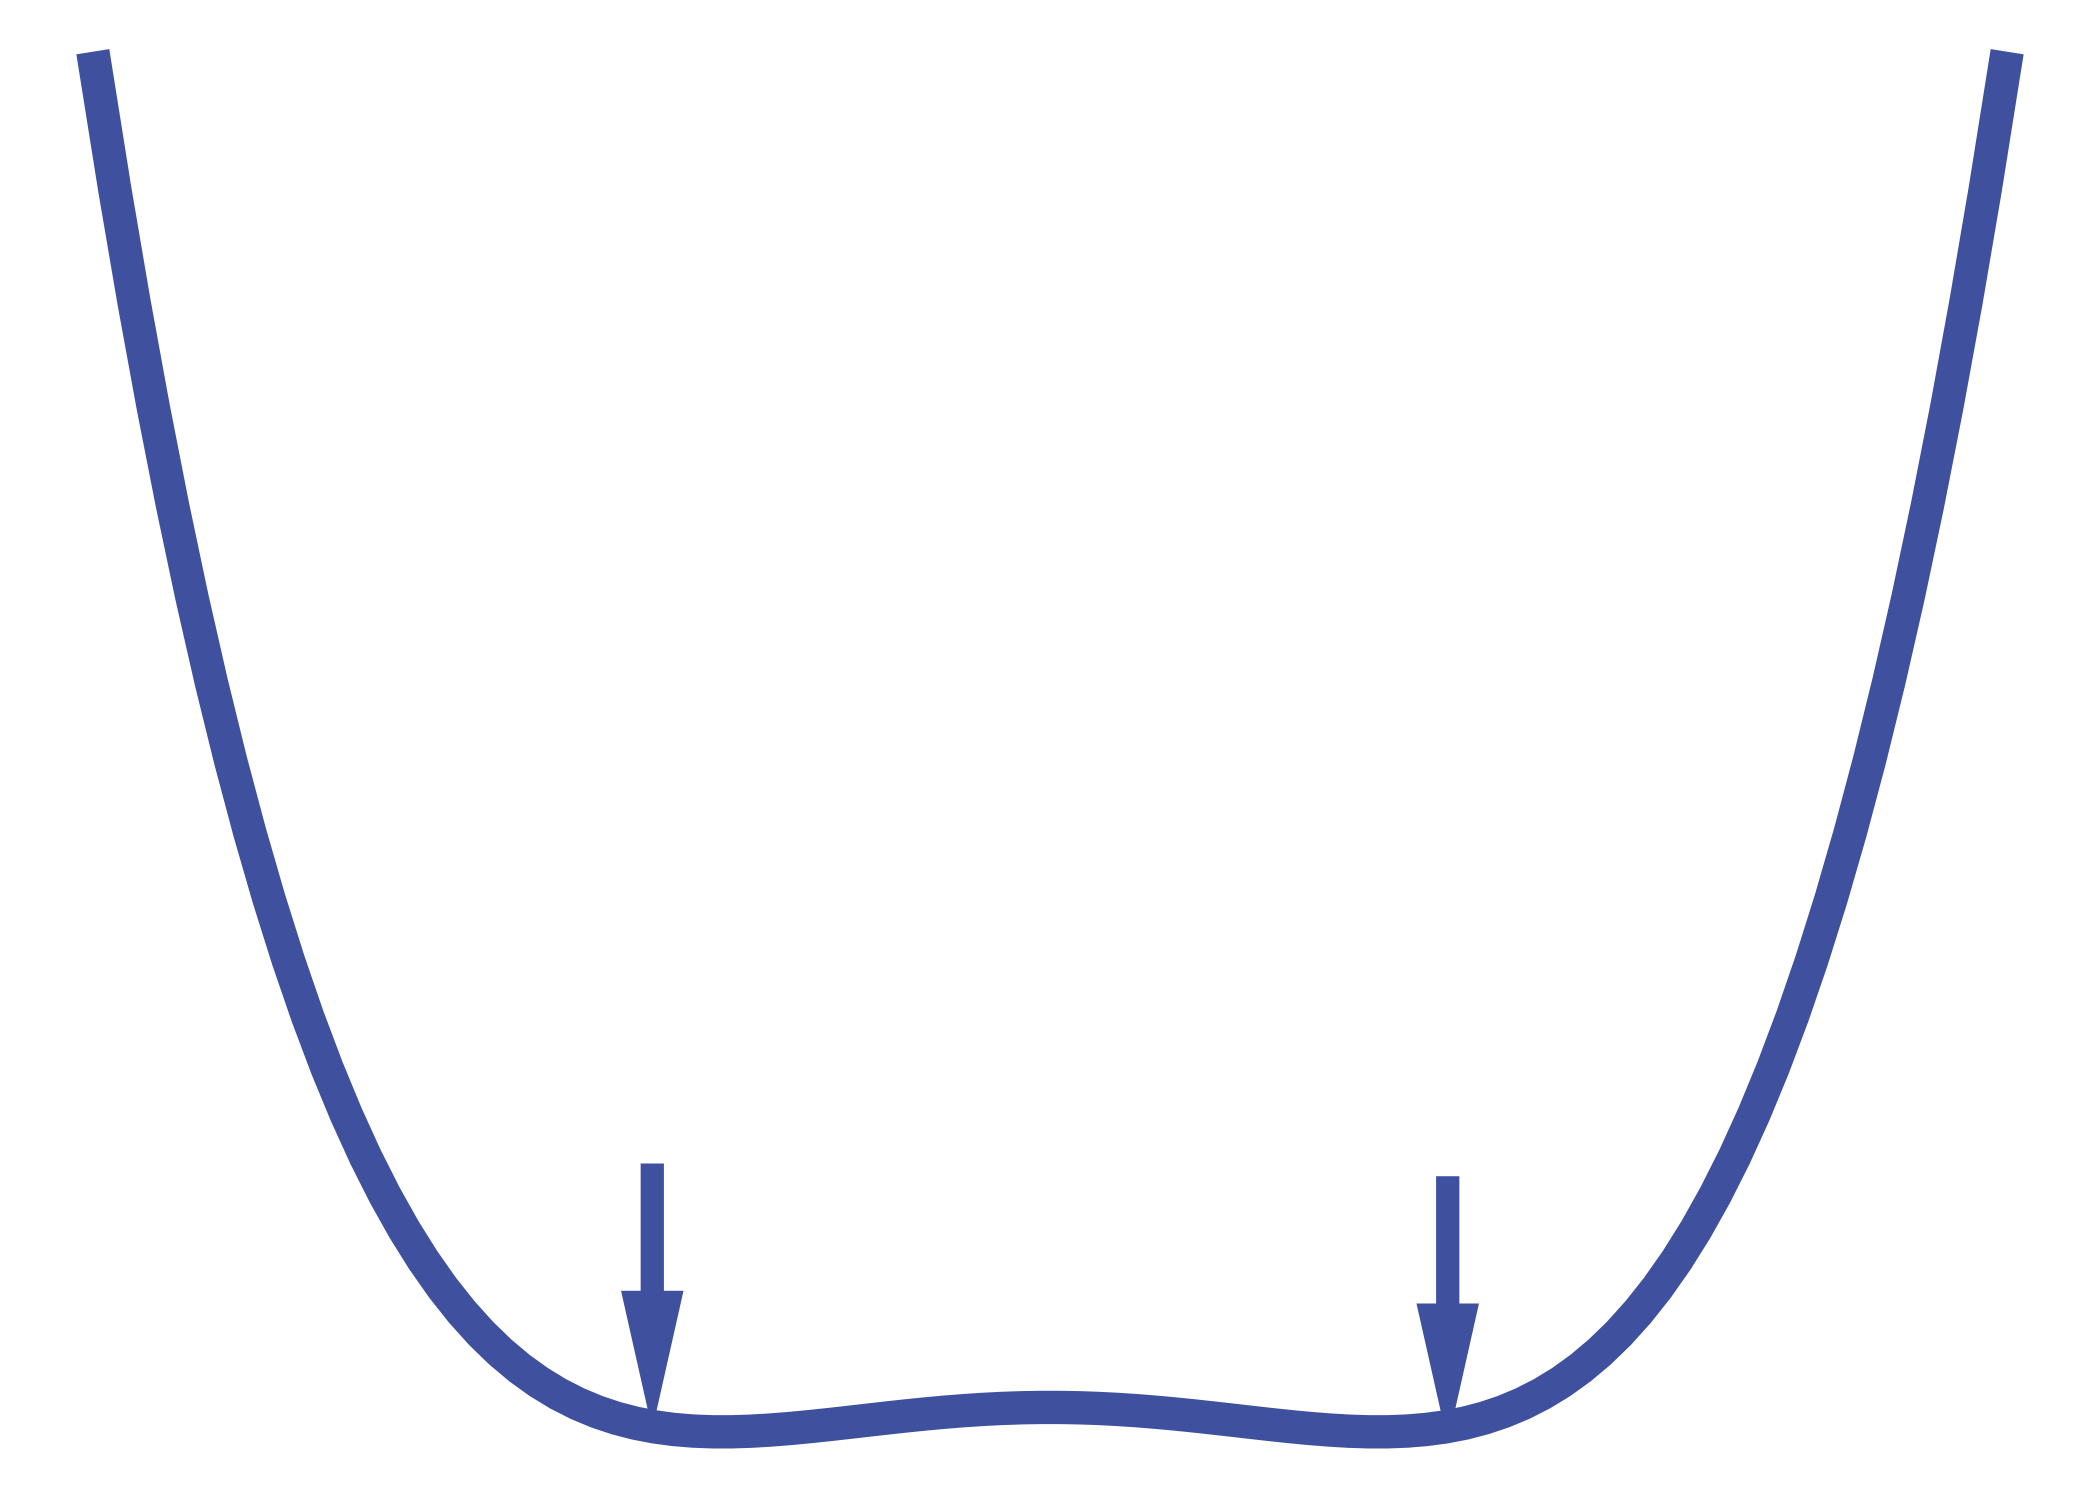
\includegraphics[width=\textwidth]{img/landau_elastic1.png}}
\only<3>{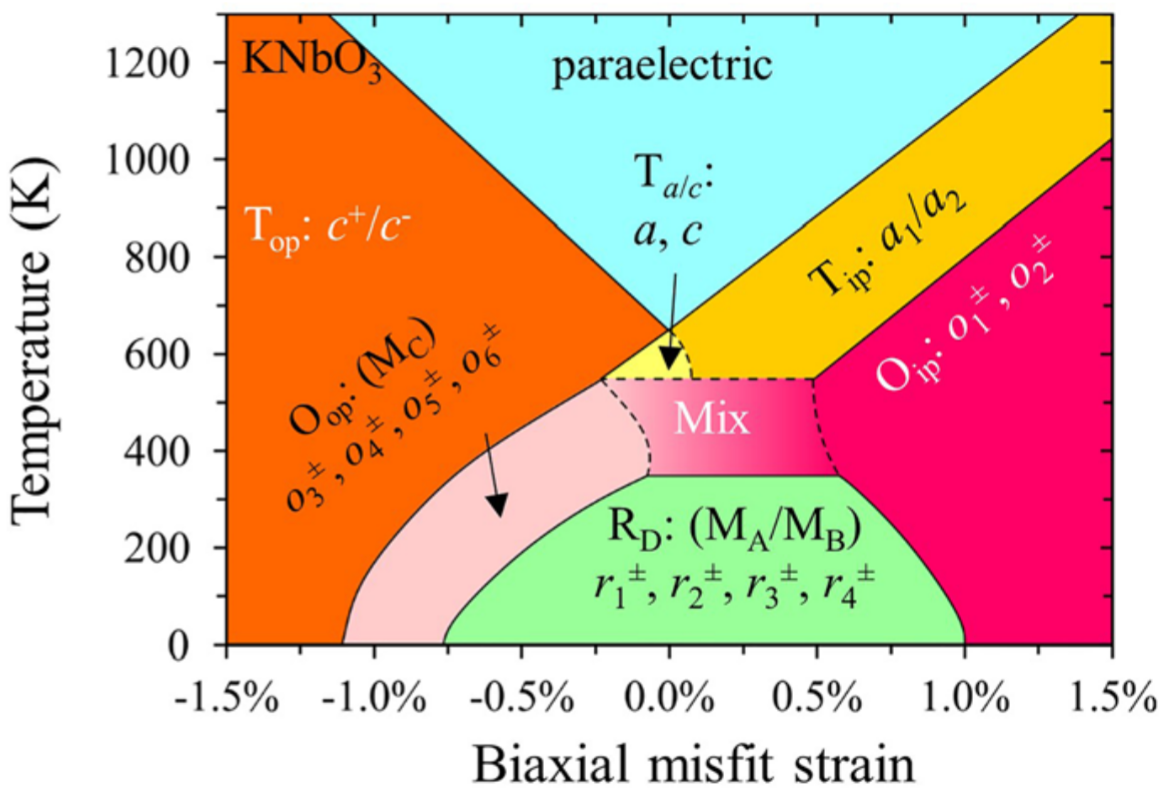
\includegraphics[width=\textwidth]{img/knn-phase-diagram.png}}
\only<4>{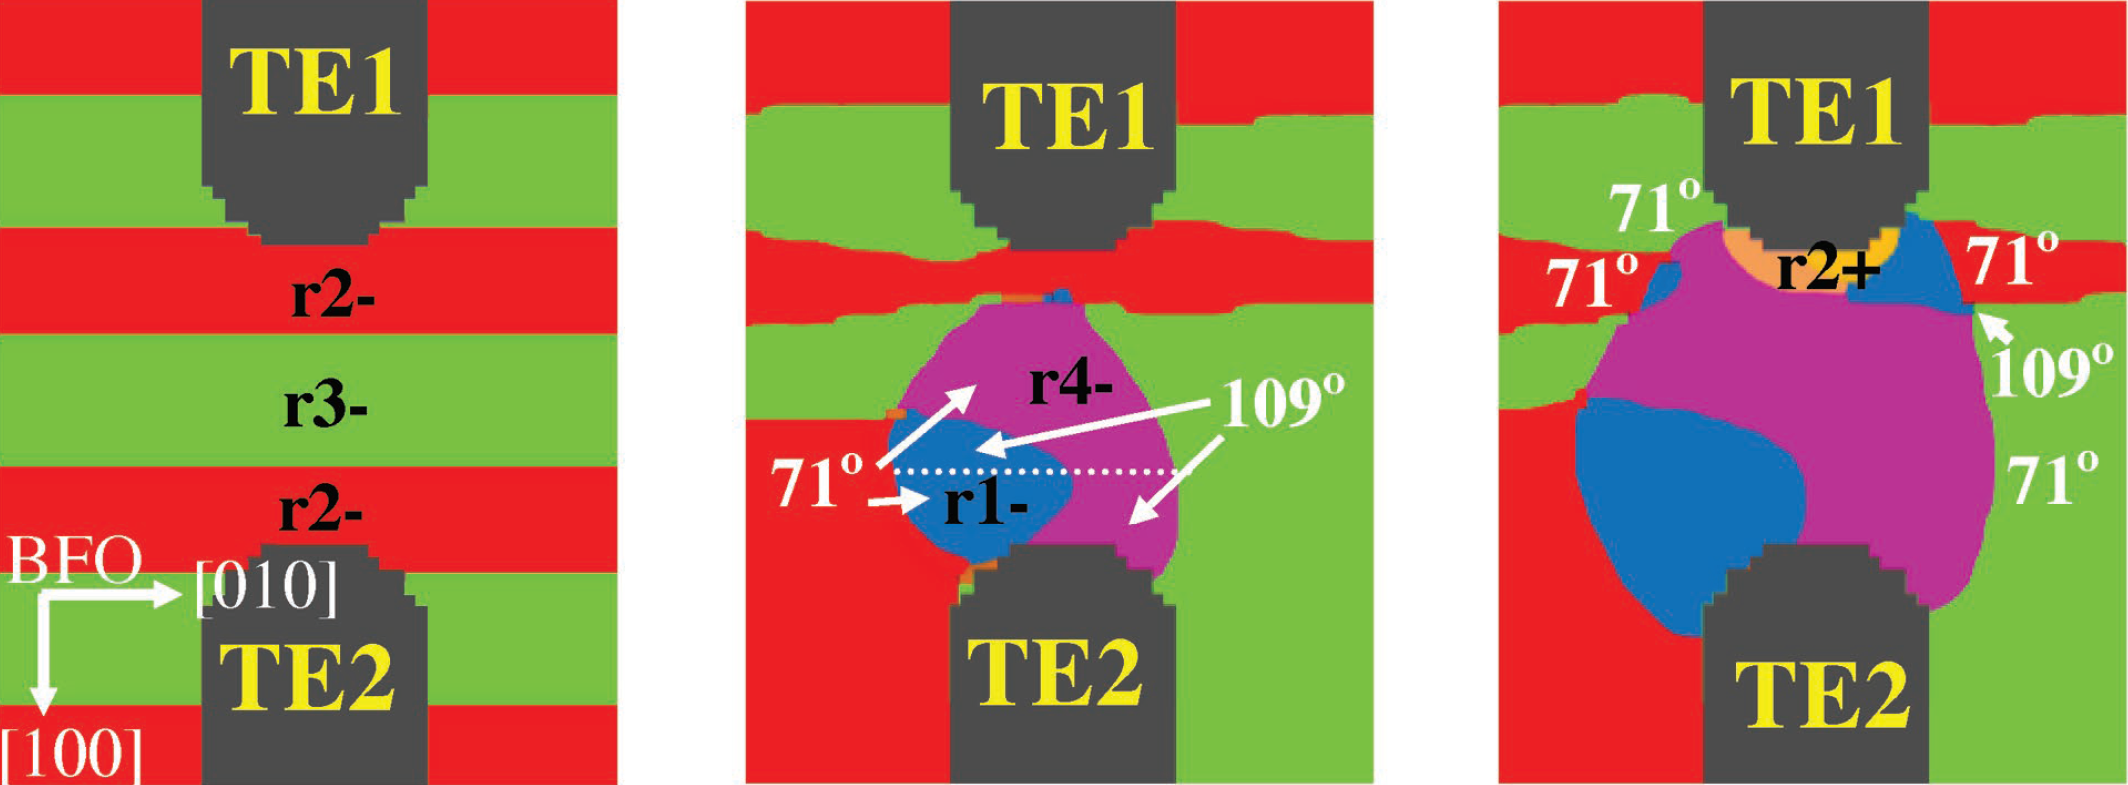
\includegraphics[width=\textwidth]{img/bfo-hierarchical.png}}
\end{columns}
\end{frame}

\begin{frame}[fragile]{Project 1: Ferroelectric -- Input: pot.in}
\begin{columns}
\column{0.5\linewidth}
\centering
\vskip 0.5cm
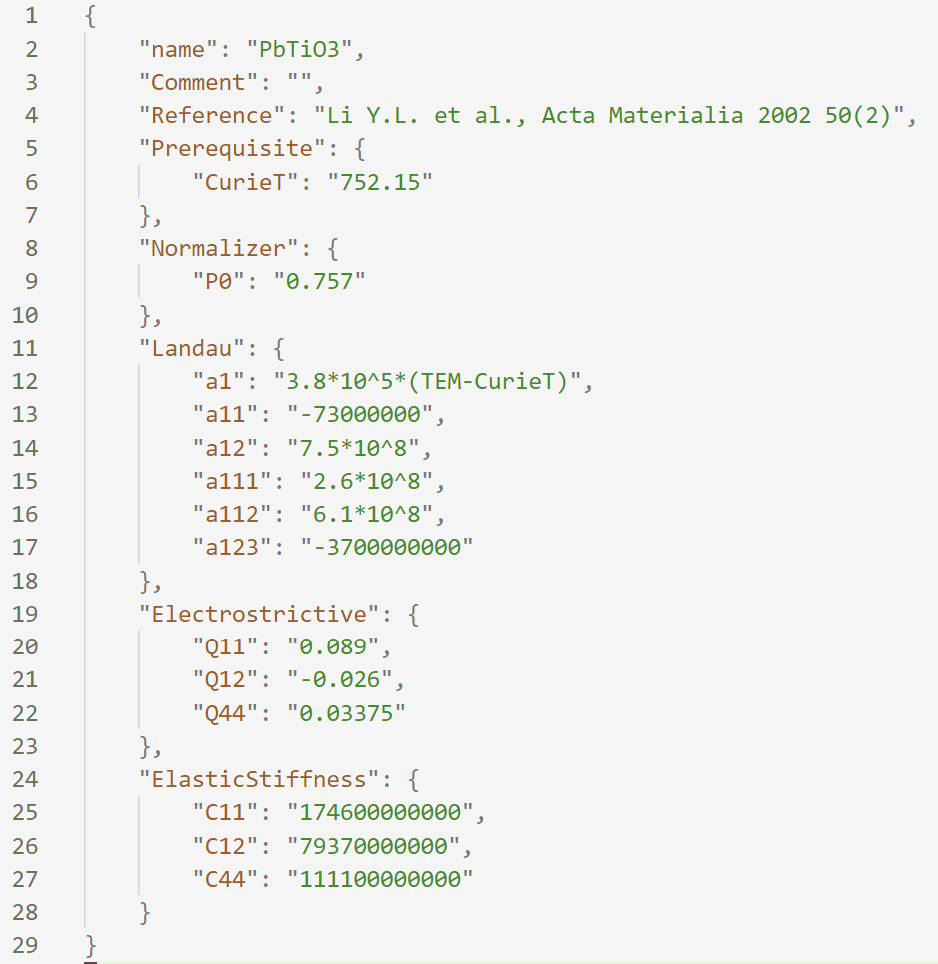
\includegraphics[width=0.9\textwidth]{img/pot.png}
\column{0.5\linewidth}
\justify
{\bf pot.in} is a json format input file for the MUPRO ferroelectric module, which feeds those necessary physical parameters into the program, such as the landau coefficient, the electrostrictive coefficient, the elastic stiffness, etc.
\end{columns}
\end{frame}

\renewcommand\fnl{}
\begin{frame}[fragile]{Project 1: Ferroelectric -- Input: input.in}
\begin{columns}
\column{0.5\linewidth}
\centering
\vskip 0.5cm
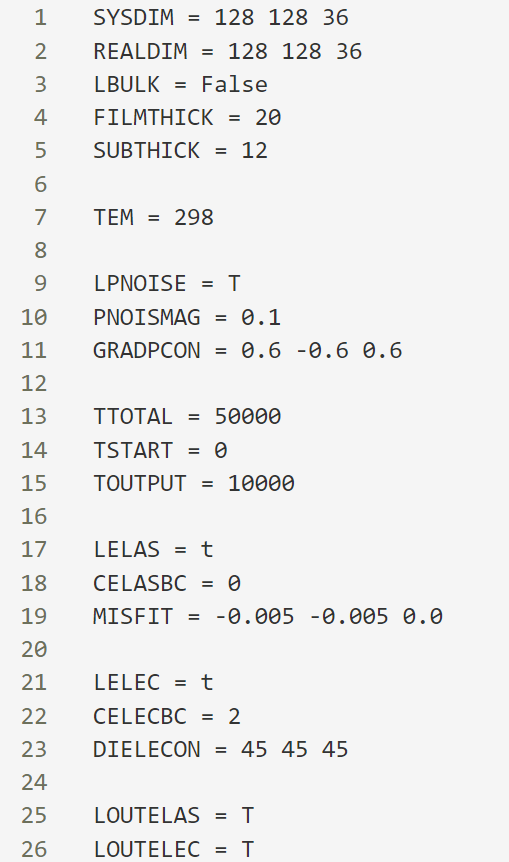
\includegraphics[width=0.6\textwidth]{img/ferro_input.png}
\column{0.5\linewidth}
\justify
{\bf input.in} is a free format input file for the MUPRO ferroelectric module. It controls how the simulation will be executed. 
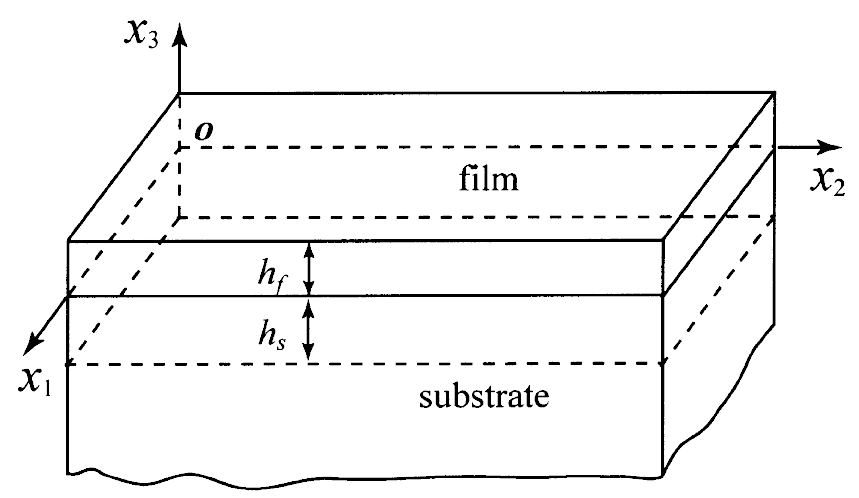
\includegraphics[width=\textwidth]{img/ferro_bc.png}
\end{columns}
\end{frame}

\begin{frame}[fragile]{Project 1: Ferroelectric -- Execution}
\begin{columns}
\column{0.5\linewidth}
\centering
\begin{lstlisting}[language=bash]
./Ferroelectric.exe # Run directly
# Or you may submit a job
\end{lstlisting}
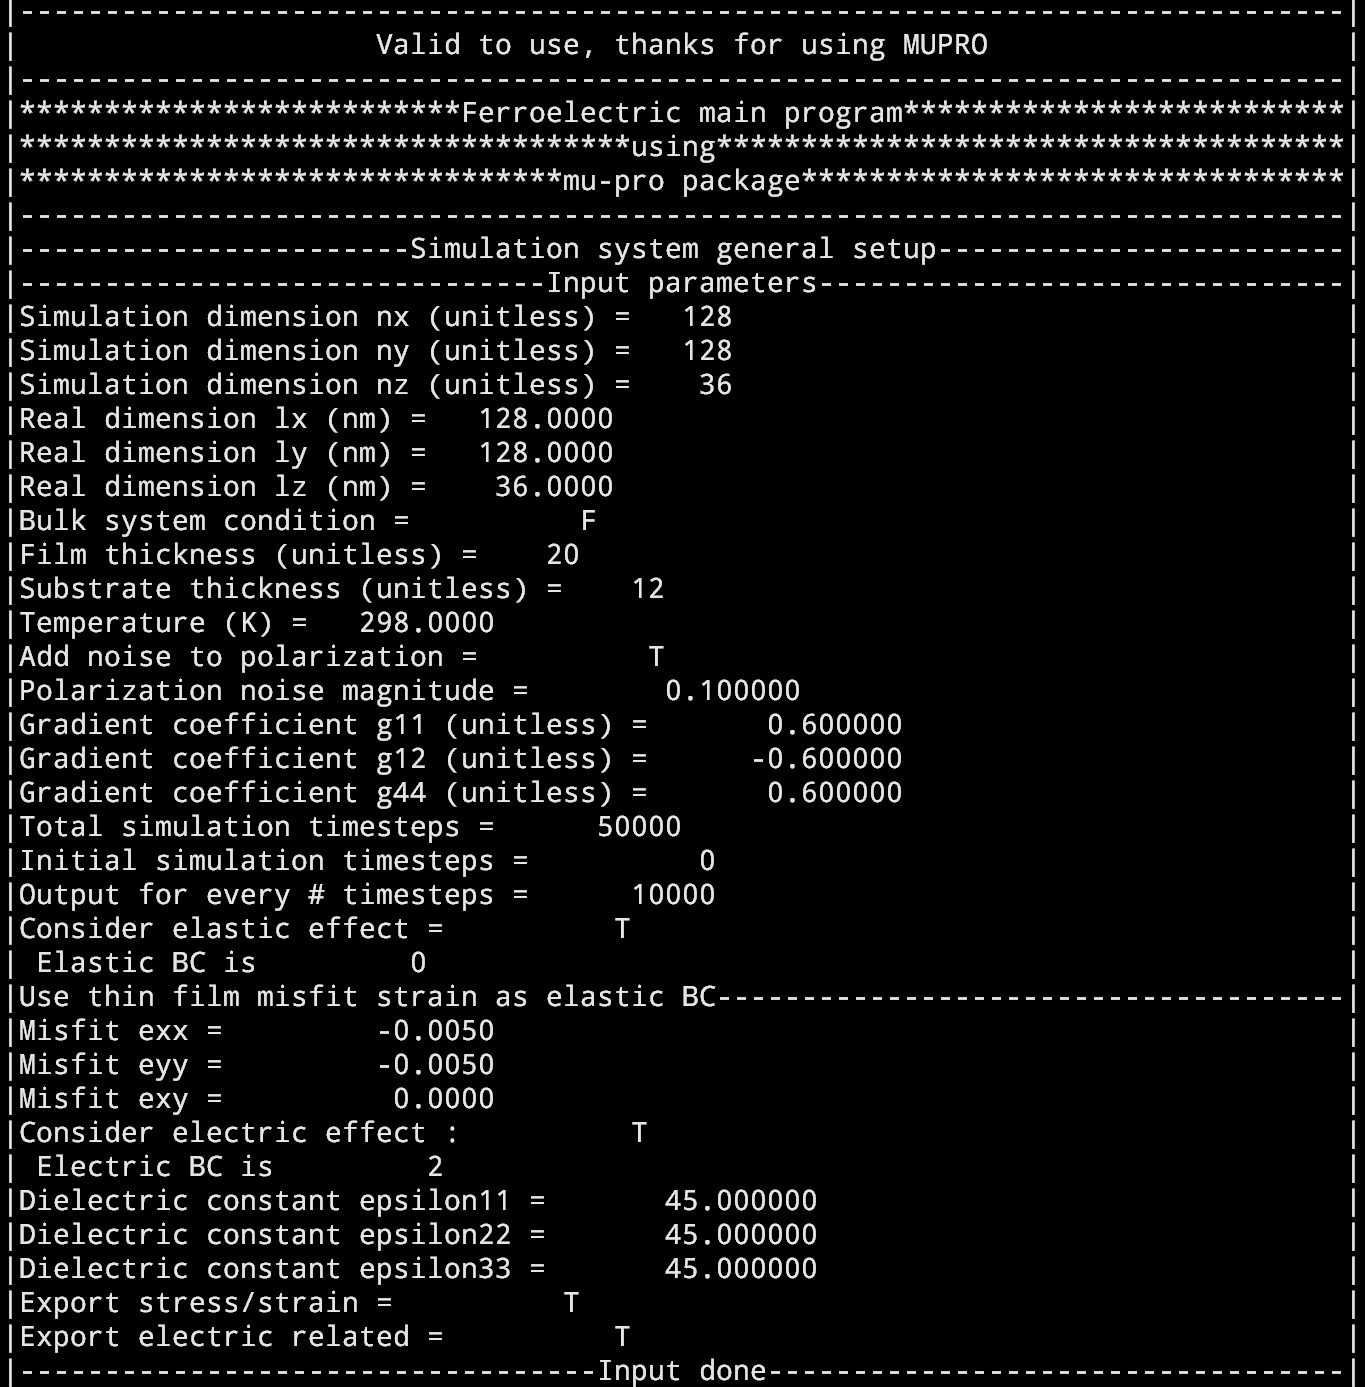
\includegraphics[height=0.85\textwidth]{img/ferro_run.png}
\column{0.5\linewidth}
\centering
\begin{lstlisting}[language=bash]
qsub ferro.pbs
qstat -u [your username]
\end{lstlisting}
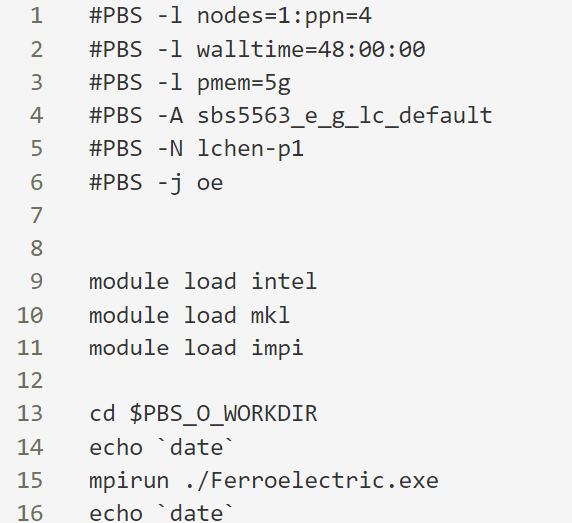
\includegraphics[height=0.85\textwidth]{img/ferro_pbs.png}
\end{columns}
\end{frame}

\subsection[Project 2: Ferromagnetic]{Project 2: Ferromagnetic}
\begin{frame}[fragile]{Project 2: Ferromagnetic -- Preparation}
\small{
\begin{lstlisting}[language=bash]
cd ..  # Go back to the pfm folder
cp -r /gpfs/group/dml129/default/matse_sc_data/lchen/project2 .
cd project2
ls
\end{lstlisting}
}
\begin{columns}
\column{0.7\linewidth}
    \begin{itemize}
        \item [parameter.in] Boundary conditions and applied external field 
        \item [magn.pbs] The PBS submission script
        \item [Magnetic.exe] The executable that we are using
    \end{itemize}
    % \vskip 0.5cm
    % Polar.in may also be defined for customizing the initial polarization distribution.
\end{columns}
\end{frame}

\begin{frame}[fragile]{Project 2: Ferromagnetic -- Input: parameter.in}
\begin{columns}
\column{0.5\linewidth}
\centering
\vskip 0.5cm
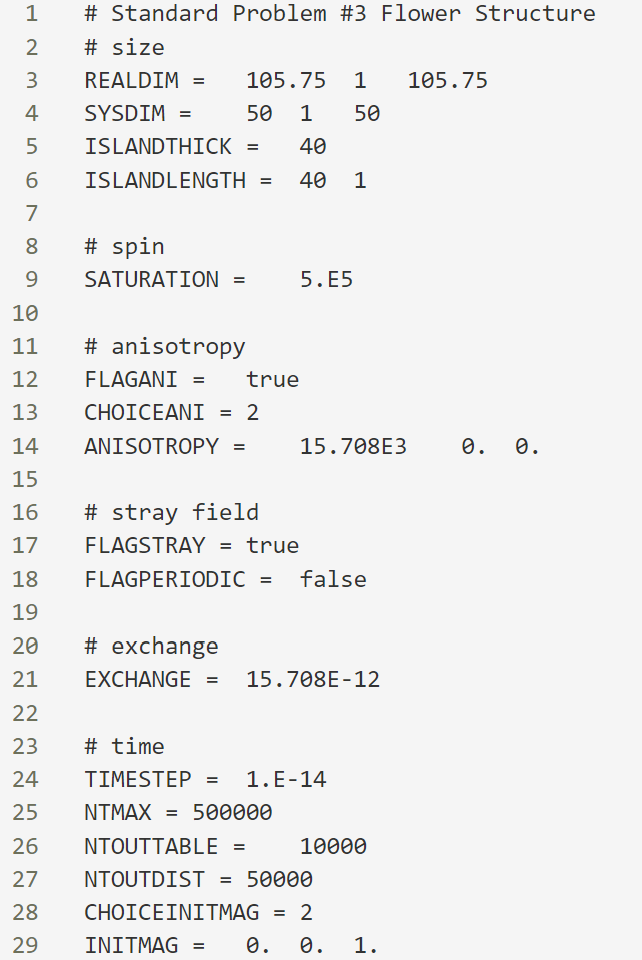
\includegraphics[width=0.7\textwidth]{img/magn_param.png}
\column{0.5\linewidth}
\justify
{\bf parameter.in} is a free format input file for the MUPRO magnetic module. It controls the simulation program.
\end{columns}
\end{frame}

\begin{frame}[fragile]{Project 2: Ferromagnetic -- Execution}
\begin{columns}
\column{0.5\linewidth}
\centering
\begin{lstlisting}[language=bash]
./Magnetic.exe
\end{lstlisting}
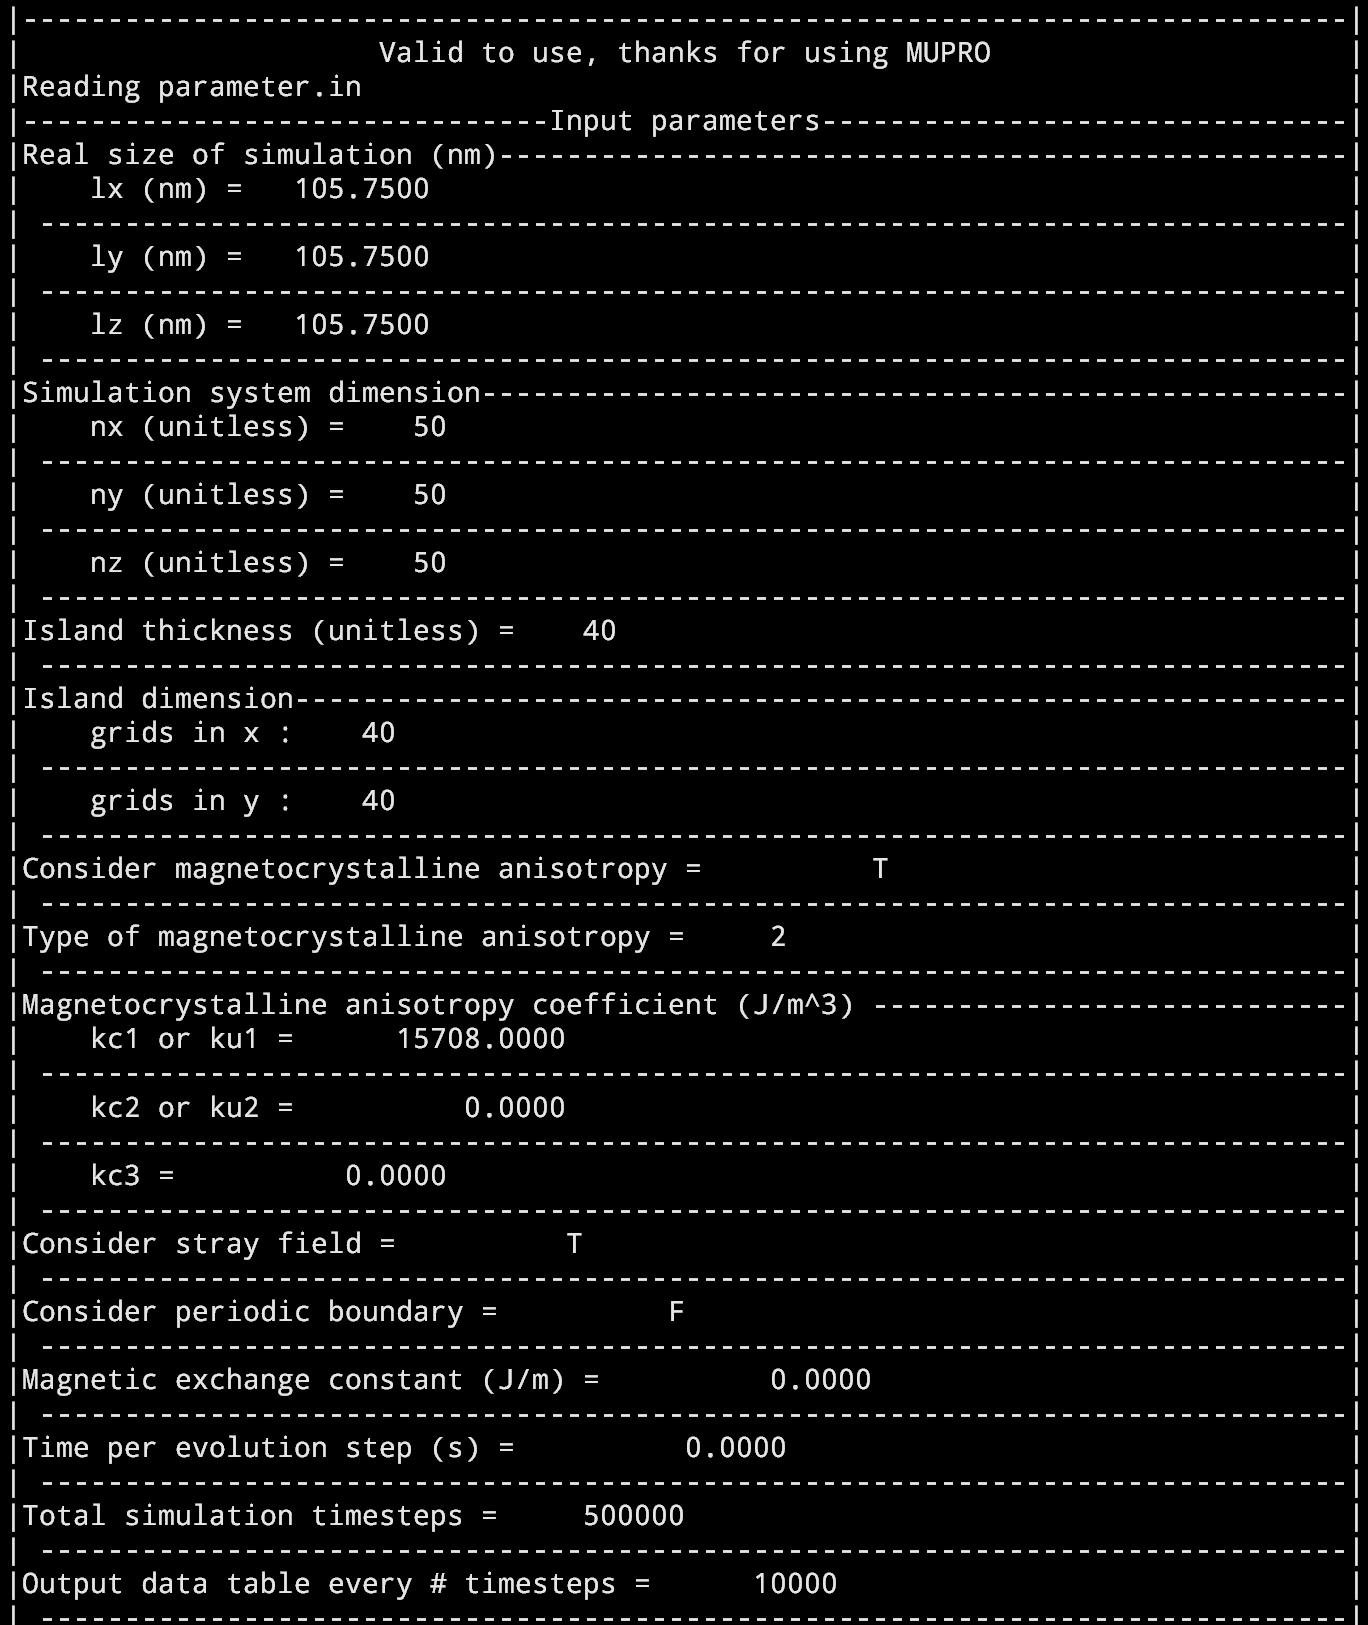
\includegraphics[height=0.85\textwidth]{img/magn_run.png}
\column{0.5\linewidth}
\centering
\begin{lstlisting}[language=bash]
qsub magn.pbs
\end{lstlisting}
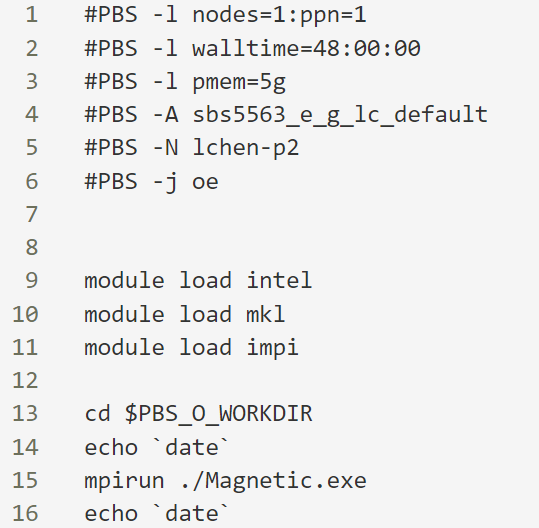
\includegraphics[height=0.85\textwidth]{img/magn_pbs.png}
\end{columns}
\end{frame}

\subsection[Project 3: Effective Property]{Project 3: Effective Property}
\begin{frame}[fragile]{Project 3: Effective Property -- Preparation}
\small{
\begin{lstlisting}[language=bash]
cd ..  # Go back to the pfm folder
cp -r /gpfs/group/dml129/default/matse_sc_data/lchen/project3 .
cd project2
ls
\end{lstlisting}
}
\begin{columns}
\column{0.7\linewidth}
    \begin{itemize}
        \item [parameter.in] Boundary conditions and applied external field 
        \item [struct.in] Composite structure setup 
        \item [eff.pbs] The PBS submission script
        \item [EffProperty.exe] The executable that we are using
    \end{itemize}
    % \vskip 0.5cm
    % Polar.in may also be defined for customizing the initial polarization distribution.
\end{columns}
\end{frame}

\begin{frame}[fragile]{Project 3: Effective Property -- Input: parameter.in}
\begin{columns}
\column{0.5\linewidth}
\centering
\vskip 0.5cm
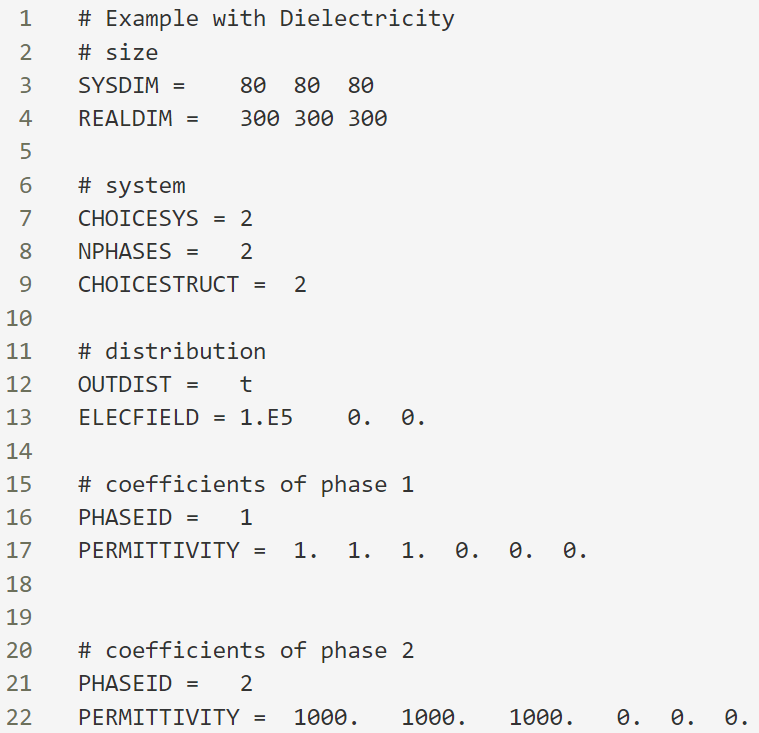
\includegraphics[width=0.8\textwidth]{img/eff_param.png}
\column{0.5\linewidth}
\justify
{\bf parameter.in} is a free format input file for the MUPRO effective property module. It controls the simulation program.
\end{columns}
\end{frame}

\begin{frame}[fragile]{Project 3: Effective Property -- Input: struct.in}
\begin{columns}
\column{0.5\linewidth}
\centering
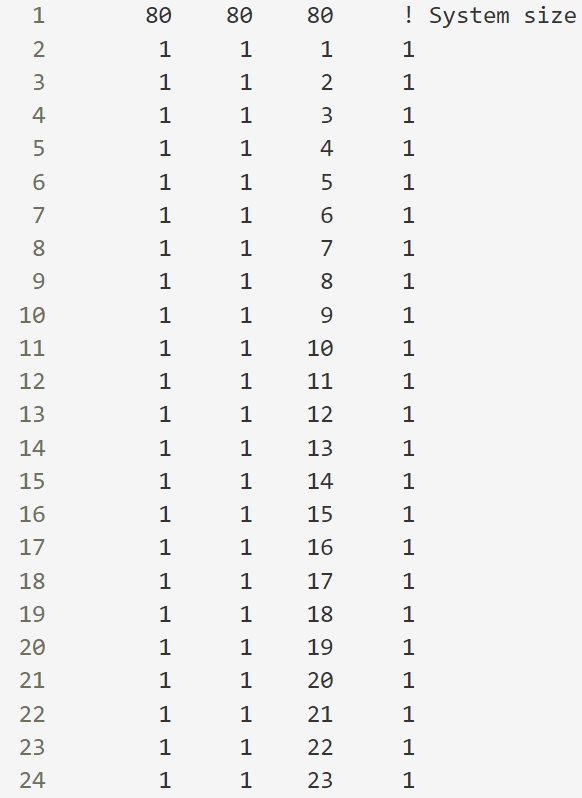
\includegraphics[width=0.7\textwidth]{img/eff_struct.png}
\column{0.5\linewidth}
\justify
{\bf struct.in} specify the composite structure.
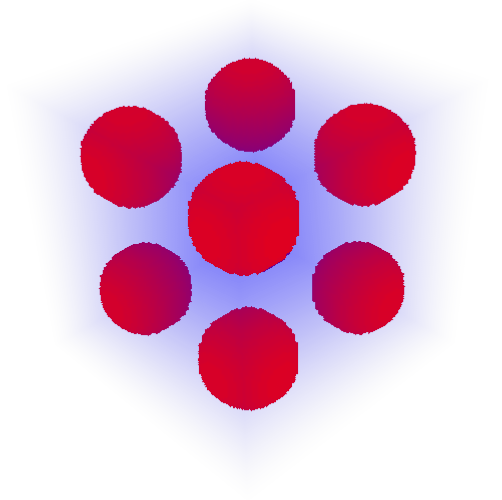
\includegraphics[width=\textwidth]{img/eff_struct_3D.png}
\end{columns}
\end{frame}

\begin{frame}[fragile]{Project 3: Effective Property -- Execution}
\begin{columns}
\column{0.5\linewidth}
\centering
\begin{lstlisting}[language=bash]
./EffProperty.exe
\end{lstlisting}
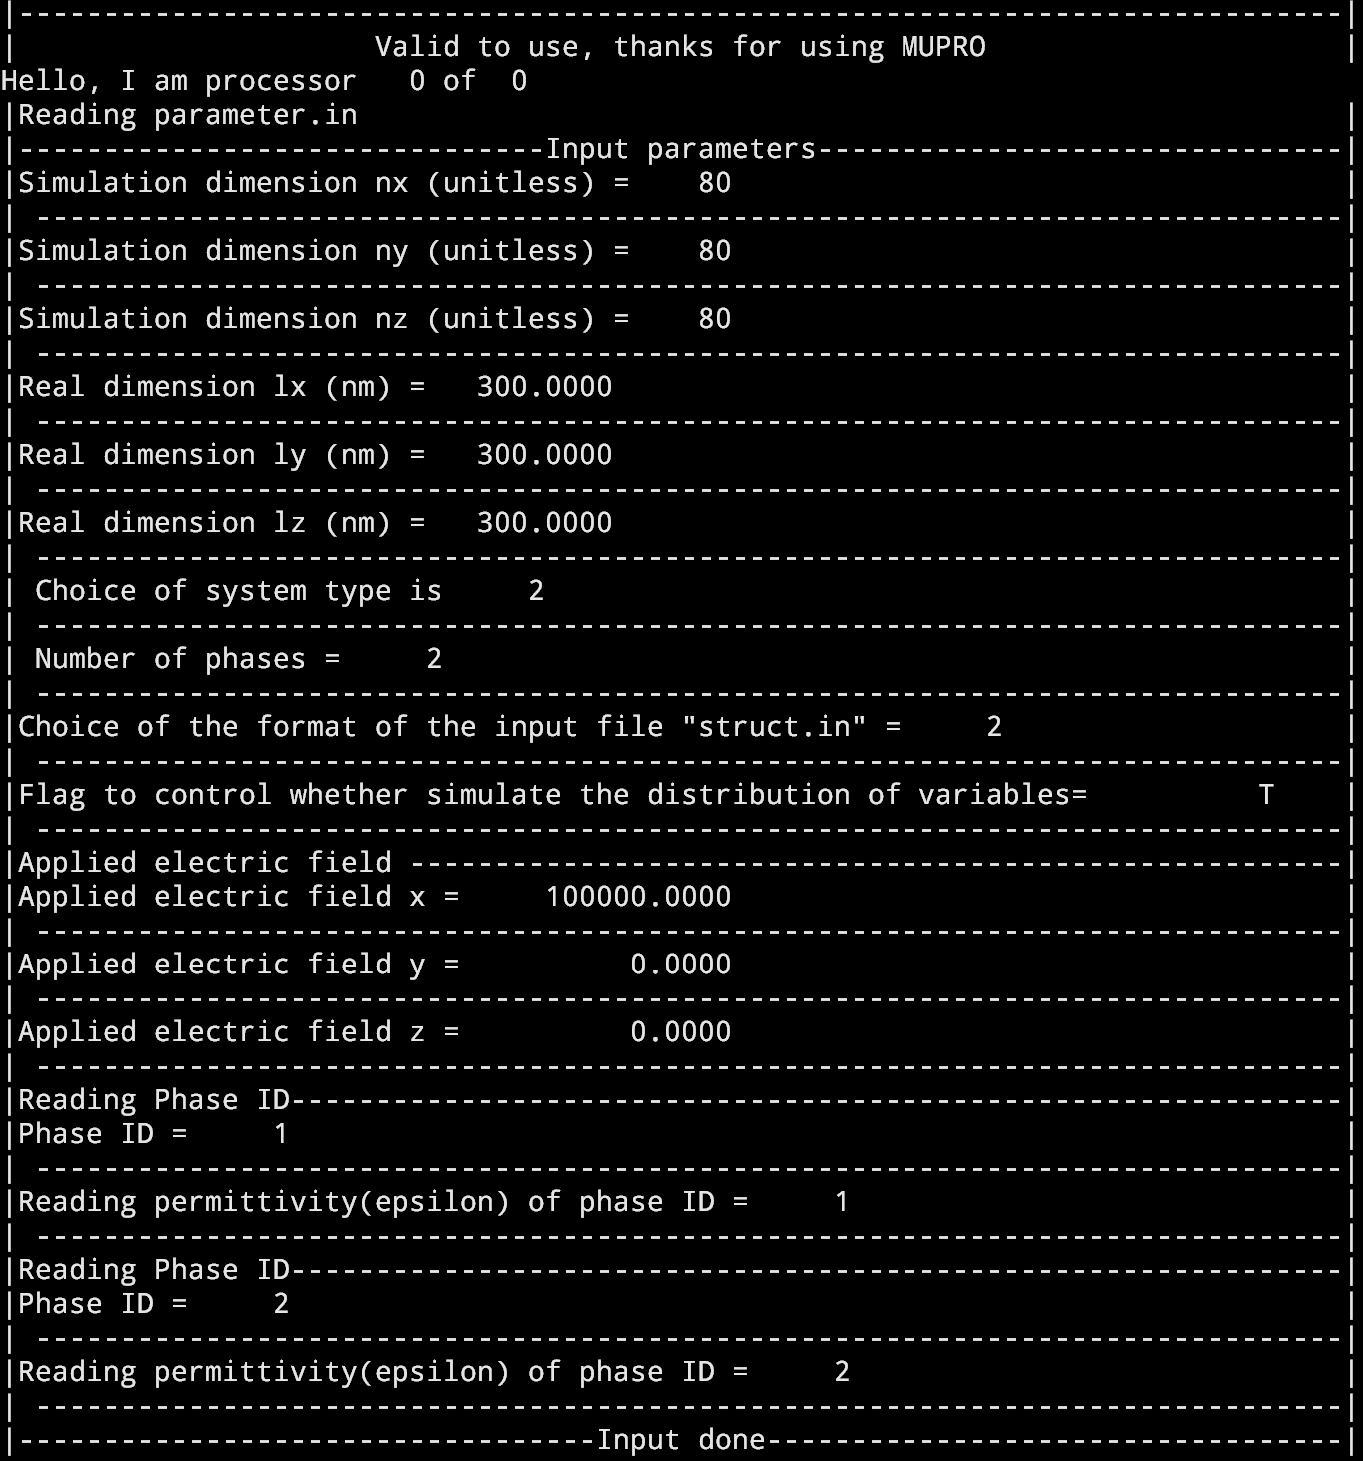
\includegraphics[height=0.85\textwidth]{img/eff_run.png}
\column{0.5\linewidth}
\centering
\begin{lstlisting}[language=bash]
qsub eff.pbs
\end{lstlisting}
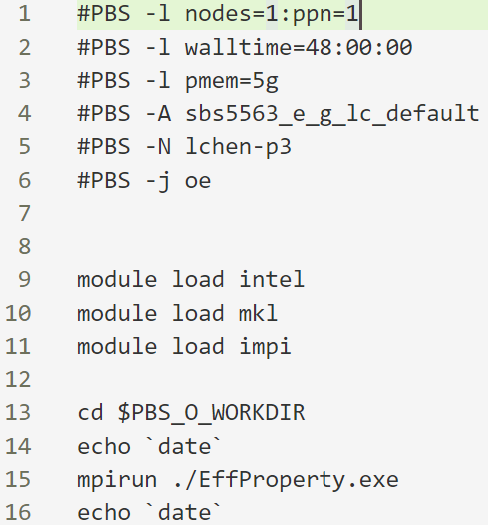
\includegraphics[height=0.85\textwidth]{img/eff_pbs.png}
\end{columns}
\end{frame}
\subsection[Visualization]{Visualization}

\begin{frame}[fragile]{Visualization: Preparation }
\begin{lstlisting}[language=bash,basicstyle=\tiny]
cd ..  # Go back to the pfm folder
export PATH=/gpfs/group/dml129/default/matse_sc_data/lchen/visualize:$PATH
export PYTHONPATH=/gpfs/group/dml129/default/matse_sc_data/lchen/visualize:$PYTHONPATH
\end{lstlisting}
The second command will give you direct access to the shell scripts we put in that folder. \\ 
The third command will enable import python file from the path as a module. 
\end{frame}

\begin{frame}[fragile]{Visualization: Domain}
\begin{lstlisting}[language=bash]
cd project1 
plot_domain.sh 1 128 1 1 1 36 0.1 0.1 0.1 Polar.00050000.dat
\end{lstlisting}
\begin{itemize}
    \item[1,2] Minimum and maximum in X direction of the plotting region
    \item[3,4] Minimum and maximum in Y direction of the plotting region
    \item[5,6] Minimum and maximum in Z direction of the plotting region
    \item[7,8,9] Threshold for vector to be considered as valid polarization
    \item[10] Data file name
\end{itemize}
\begin{lstlisting}[language=bash]
display Apersp_P_Polar.00050000.png
\end{lstlisting}
\end{frame}

\begin{frame}[fragile]{Visualization: 2D}
\begin{lstlisting}[language=bash]
cd ../project3  
plot_2ds.sh 1 80 20 20 1 80 3 eleField.00000000.dat
\end{lstlisting}
\begin{itemize}
    \item[1,2] Minimum and maximum in X direction of the plotting region
    \item[3,4] Minimum and maximum in Y direction of the plotting region
    \item[5,6] Minimum and maximum in Z direction of the plotting region
    \item[7] The column of the data file to be plotted
    \item[8] Data file name
\end{itemize}
\begin{lstlisting}[language=bash]
display fig2ds_eleField.00000000_4_80.png
\end{lstlisting}
\end{frame}

\begin{frame}[fragile]{Visualization: VTK}
\begin{lstlisting}[language=bash]
cd ../project2
python
\end{lstlisting}
Now in the python console, type the following commands
\begin{lstlisting}[language=python]
import nt_vtk  # a module for data conversion
data = nt_vtk.Data("magnt.00500000.dat",nt_vtk.SCALAR)
data.get_vtk_file('magnt.00500000.vtk')
# You can also convert to numpy array using data.get_np_array()
\end{lstlisting}
Or you may put the above commands into a file, such as data.py run it as below\\
\begin{lstlisting}[language=bash]
python data.py
\end{lstlisting}
Next, we will use Paraview to visualize the vtk file.
\begin{lstlisting}[language=bash]
module load paraview
paraview
\end{lstlisting}
\end{frame}

\begin{frame}{Visualization: VTK}
\centering
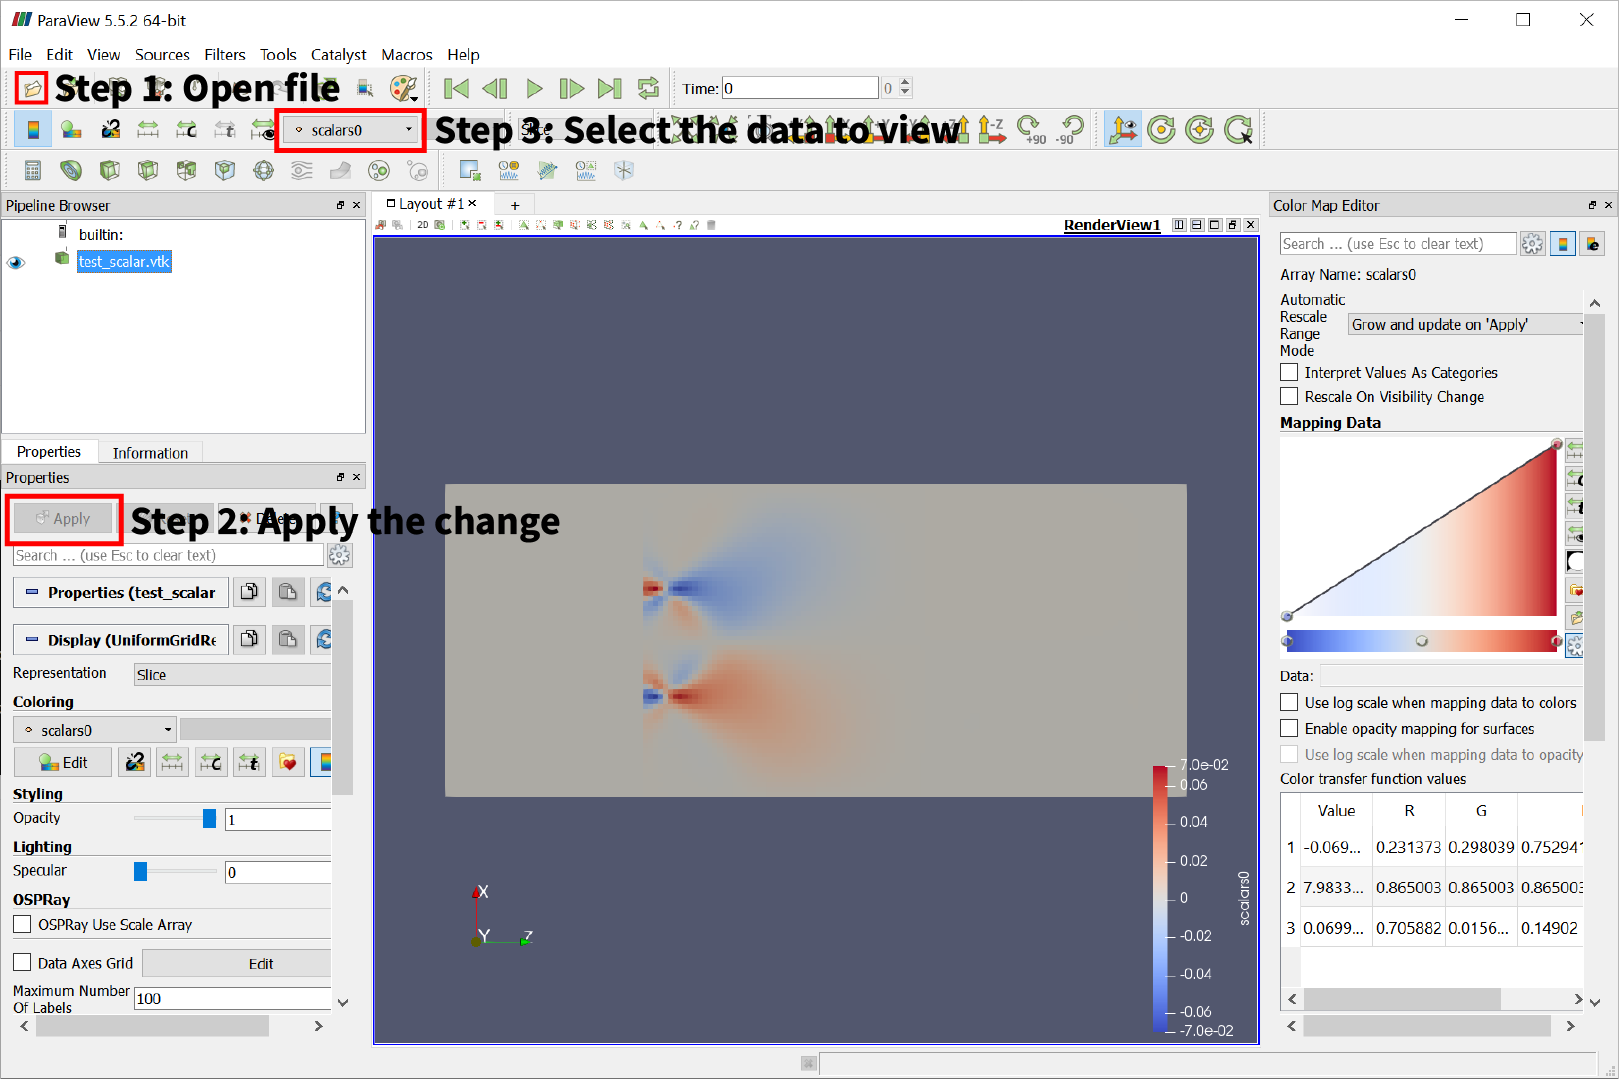
\includegraphics[width=0.8\textwidth]{img/Scalar.png}
\end{frame}

\section[Part Two: Exercises]{Part Two: Exercises}
\begin{frame}[fragile]{Get the doc}
\begin{lstlisting}[language=bash]
cd ..  # Go back to the pfm folder
cd doc
xpdf [the pdf name you want to open]
\end{lstlisting}
Read the documentation for information of the {\bf keywords} you may use for each program.
\end{frame}
\subsection[Exercise 1: Ferroelectric]{Exercise 1: Ferroelectric}
\begin{frame}{Exercise 1: Ferroelectric}
In project 1, we have a thin film setup with 0 misfit strain. Please modify the input.in file and run simulations with compressive (-0.5\%) and tensile (0.5\%) biaxial misfit strain.

Change {\bf MISFIT}.
\end{frame}
\subsection[Exercise 2: Ferromagnetic]{Exercise 2: Ferromagnetic}
\begin{frame}{Exercise 2: Ferromagnetic}
In project 2, we have got a flower structure. For exercise 2, please modify the parameter.in file to obtain a vortex structure. 

Set {\bf CHOICEINITMAG} to be {\bf 3}, {\bf INITMAG} to be {\bf 0 -1 0}
\end{frame}
\subsection[Exercise 3: Effective Property]{Exercise 3: Effective Property}
\begin{frame}{Exercise 3: Effective Propert}
In project 3, we have computed the effective dielectric permittivity. For exercise 3, please modify the parameter.in file to calculate the effective thermal conductivity, for the following setup.

\begin{itemize}
    \item {\bf CHOICESYS} set to {\bf 8}
    \item {\bf TEMGRAD} set to {\bf 1.E4 0 0}
    \item {\bf THERMCOND} of phase 1 to {\bf 0.2 0.2 0.2 0 0 0}
    \item {\bf THERMCOND} of phase 2 to {\bf 200 200 200 0 0 0}
\end{itemize}

\end{frame}


\end{document}
